\documentclass[a4paper, czech]{article}

\usepackage[czech]{babel}
\usepackage{indentfirst}
\usepackage{graphicx}
\usepackage{float}
\usepackage[margin=1.5cm]{geometry}
\usepackage{booktabs}
\usepackage{amsmath}
\usepackage{xcolor}
\usepackage{multirow}
\usepackage{tabularray}
\usepackage{bold-extra}
\usepackage{circuitikz}
\usetikzlibrary{decorations, decorations.pathreplacing, decorations.pathmorphing}
\usepackage{caption}
\usepackage{subcaption}
\usepackage[utf8]{inputenc}

\begin{document}
\begin{table}[H]
    \centering
    \begin{tblr}{
        cell{1}{1} = {c = 2, r = 4}{c}, % Logo
        cell{1}{4} = {c = 3}{c}, % Předmět
        cell{2}{4} = {c = 3}{c}, % Jméno
        cell{3}{4} = {}{c}, % Ročník
        cell{3}{6} = {}{c}, % Studijní skupina
        cell{4}{4} = {}{c}, % Spolupracoval
        cell{4}{6} = {}{c}, % Mereno dne
        cell{5}{1} = {c = 2}{55mm}, % Kontroloval
        cell{5}{3} = {c = 2}{55mm}, % Hodnoceni
        cell{5}{5} = {c = 2}{55mm}, % Dne
        cell{6}{2} = {c = 5}{}, % Nazev ulohy
        cell{7}{1} = {}{c}, % Číslo úlohy
        cell{7}{2} = {c = 5}{c}, % Název úlohy
        vline{1,2,7} = {1.2pt},
        vline{3,5},
        hline{1,5,6,8} = {1.2pt},
        hline{2,3,4}
        }
        
\includegraphics{logo_fekt.png} & & \textsuperscript{Předmět} & \large \textbf{Měření v audiotechnice} \\
             & & \textsuperscript{Jméno} & \large \textbf{Karolína Šebestová} \\
             & & \textsuperscript{Ročník} & \large \textbf{3.} & \textsuperscript{Studijní skupina} & \large \textbf{St 14:00} \\
             & & \textsuperscript{Spolupracoval} & \large \textbf{Filip Kokavec} & \textsuperscript{Měřeno dne} & \large \textbf{13.11.2024} \\
        \textsuperscript{Kontroloval} & & \textsuperscript{Hodnocení} & & \textsuperscript{Dne} \\
        \textsuperscript{Číslo úlohy} & \textsuperscript{Název úlohy} \\
        \Large \textbf{7A} & \Large \textsc{\textbf{Měření statické hysterezní smyčky}} \\
    \end{tblr}
\end{table}

\section{Zadání}

\begin{itemize}
    \item Obeznamte se s měřením křivek prvotní magnetizace a hysterezních smyček integrační metodou při stejnosměr- ném magnetování.
    \item Změřte statickou hysterezní smyčku předložených feromagnetických jader pomocí automatizovaného pracoviště.
\end{itemize}

\section{Teoretický úvod}

Hysterezní charakteristika je graf závislosti magnetické indukce $B$ na na intenzitě magnetického pole $H$.
Stejnosměrné magnetování nastává v případě, kdy se intenzita magnetického pole a magnetická indukce v materiálu mění tak pomalu, že se neuplatňují vlivy rušivých vířivých proudů.
Další zpomalování změny intenzity magnetického pole a magnetické indukce již nemá vliv na tvar měřené charakteristiky.

\begin{itemize}
    \item \textbf{Křivka prvotní magnetizace} - je důležité dokonalé odmagnetování, popisuje magnetizaci vzorku pouze jedním směrem.
    \item \textbf{Statická maximální hysterezní smyčka} - je to závislost popisující pomalé magnetizační cykly. Průsečík s osou magnetické indukce udává hodnoty remanentní indukce $B_\text{r}$. Průsečík s osou intenzity magnetického pole udává hodnotu koercivní síly $H_\text{c}$. Maximální hysterezní smyčka je taková, kde se při zvyšování hodnoty $H_\text{m}$ již nezvyšují polohy průsečíků $B_\text{r}$ a $H_\text{c}$. Hysterezní ztráty v materiálu jsou úměrné velikosti plochy této smyčky.
    \item \textbf{Magneticky měkký/tvrdý materiál} - udává šířka hysterezní smyčky
\end{itemize}

\begin{figure}[H]
    \centering
    \begin{circuitikz}[decoration={coil, segment length=0.7mm, amplitude=2mm}]
        % Zdroj magnetizačního proudu
        \draw (0,0) node[align=center, draw, rectangle, inner xsep=7.5](ZMP){Zdroj\\magnetizačního\\proudu}
        (ZMP.east) +(0,0.5) coordinate(ZMP+) (ZMP.east) +(0,-0.5) coordinate(ZMP-)
        (ZMP+) to[short, f=$i_m(t)$] +(1.5,0) coordinate(ZMP+)
        (ZMP-) to +(1.5,0) coordinate(ZMP-)

        % Měřené jádro
        (ZMP.east) +(2.5,0) circle[radius=0.8] circle[radius=0.5] coordinate(toroid);
        \draw[decorate, dash pattern=on 19.6pt off 8.05pt,dash phase=24.05pt] (toroid)
        +(125:0.63) coordinate(torIN1) arc[start angle=125,end angle=242,radius=0.63] coordinate(torIN2);
        \draw[decorate, dash pattern=on 19.6pt off 8.05pt,dash phase=24.05pt] (toroid)
        +(295:0.63) coordinate(torOUT2) arc[start angle=295,end angle=412,radius=0.63] coordinate(torOUT1);

        \draw (torIN2) to +(225:0.3) coordinate(torIN2) node[label=below:$N_1$]{};
        \draw (torIN1) +(135:0.165) to +(135:0.3) coordinate(torIN1);
        \draw (torOUT2) +(310:0.165) to +(310:0.3) coordinate(torOUT2) node[label=below:$N_2$]{};
        \draw (torOUT1) to +(40:0.3) coordinate(torOUT1);

        \draw (toroid) +(0,1.1) node[]{Měřené jádro};

        \draw (ZMP+) to (ZMP+ |- torIN1) to (torIN1);
        \draw (ZMP-) to (ZMP- |- torIN2) to (torIN2);

        % Elektronický Wb-metr
        \draw (toroid) +(2,0) node[align=center, draw, rectangle, anchor=west, minimum height=1.3cm, inner xsep=7.5](webrmetr){Elektronický\\Wb-metr}
        (webrmetr.west) +(0,0.5) node[ocirc](wbin+){} +(0,-0.5) node[ocirc](wbin-){}
        (webrmetr.east) +(0,0.5) node[ocirc](wbout+){} +(0,-0.5) node[ocirc](wbout-){}
        (wbin+) to +(-1,0) coordinate(X) to (X |- torOUT1) to (torOUT1)
        (wbin-) to +(-1,0) coordinate(X) to (X |- torOUT2) to (torOUT2)
        (webrmetr.west) +(-0.5,0) node[]{$u_1(t)$}
        (webrmetr.east) +(0.5,0) node[]{$u_2(t)$};

        % Měřící ústředna
        \draw (toroid) +(0,-3) node[align=center, draw, rectangle, minimum height=1.3cm, inner xsep=7.5](ustredna){Měřící\\ústředna}
        (ustredna.east) +(0,0.25) coordinate(us1) +(0,-0.25) coordinate(us2);
        \draw[-{Triangle[scale=2]}] (ustredna.north) to +(0,0.5) coordinate(X) to (X -| ZMP.south) to (ZMP.south);
        \draw (wbout+) to +(1,0) coordinate(X) to (X |- us2) to (us2)
        (wbout-) to +(0.5,0) coordinate(X) to (X |- us1) to (us1);

        % PC
        \draw (ustredna.west) +(-1,0) node[align=center, draw, rectangle, minimum height=1cm, inner xsep=7.5, anchor=east](pc){PC};
        \draw[{Triangle[scale=2]}-{Triangle[scale=2]}] (pc.east) to (ustredna.west);
    \end{circuitikz}
    \caption{Zapojení úlohy pro automatické měření statické hysterezní smyčky}
\end{figure}

\section{Výsledky měření}

\subsection{Tabulky}

\begin{table}[H]
    \catcode`\-=12
    \centering
    \caption{Naměřené hodnoty feromagnetického vzorku pro statickou hysterezní smyčku}
    \begin{tabular}{cccccccccc}
        \toprule
        \multirow{3}{*}{$H_m = 100\,\text{A} \cdot \text{m}^{-1}$} & $B_{\text{m}}$       & $H_{\text{m}}$       & $B_{\text{r}}$       & $H_{\text{c}}$        & $\Delta_{B1}$     & $\Delta_{H1}$       & $\Delta_{B2}$      & $\Delta_{H2}$        & $\mu_{\text{max}}$         \\
        \cmidrule(rl){2-2}
        \cmidrule(rl){3-3}
        \cmidrule(rl){4-4}
        \cmidrule(rl){5-5}
        \cmidrule(rl){6-6}
        \cmidrule(rl){7-7}
        \cmidrule(rl){8-8}
        \cmidrule(rl){9-9}
        \cmidrule(rl){10-10}
                                        & T        & $\text{A} \cdot \text{m}^{-1}$    & T        & $\text{A} \cdot \text{m}^{-1}$     & T       & $\text{A} \cdot \text{m}^{-1}$     & T        & $\text{A} \cdot \text{m}^{-1}$      & -            \\
        \cmidrule(rl){2-10}
                                        & 1,226    & 100      & 0,966\,6   & 16        & -       & -         & -        & -          & 20\,631,96     \\
        \cmidrule[0.8pt](rl){1-10}
        \multirow{2}{*}{Konstanty}      & \multicolumn{3}{l}{$d_1$ = 70\,mm} & \multicolumn{3}{l}{$d_2$ = 110\,mm} & \multicolumn{3}{l}{$h$ = 20\,mm}      \\
                                        & \multicolumn{3}{l}{$N_1$ = 100}   & \multicolumn{3}{l}{$N_2$ = 50}     & \multicolumn{3}{l}{$k_\phi$ = 3,0\,$\text{mWb} \cdot \text{V}^{-1}$} \\
        \bottomrule
    \end{tabular}
\end{table}

\subsection{Grafy}

\begin{figure}[H]
    \centering
    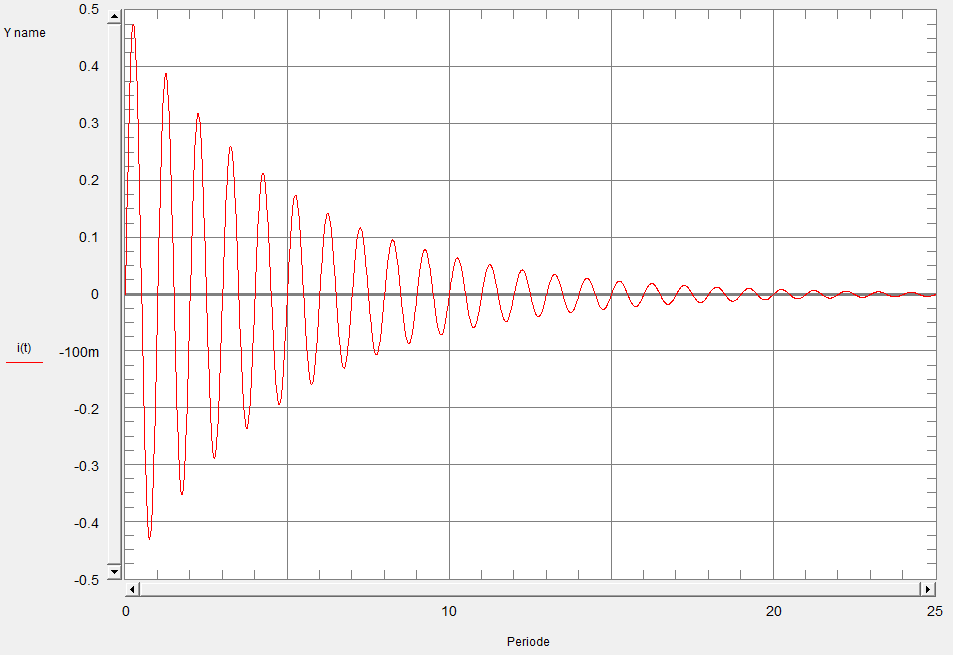
\includegraphics[width=0.9\textwidth]{demag.png}
    \caption{Průběh demagnetizace měřeného jádra}
\end{figure}

\begin{figure}[H]
    \centering
    \begin{circuitikz}
        \draw (0,0) node[](magKrivka){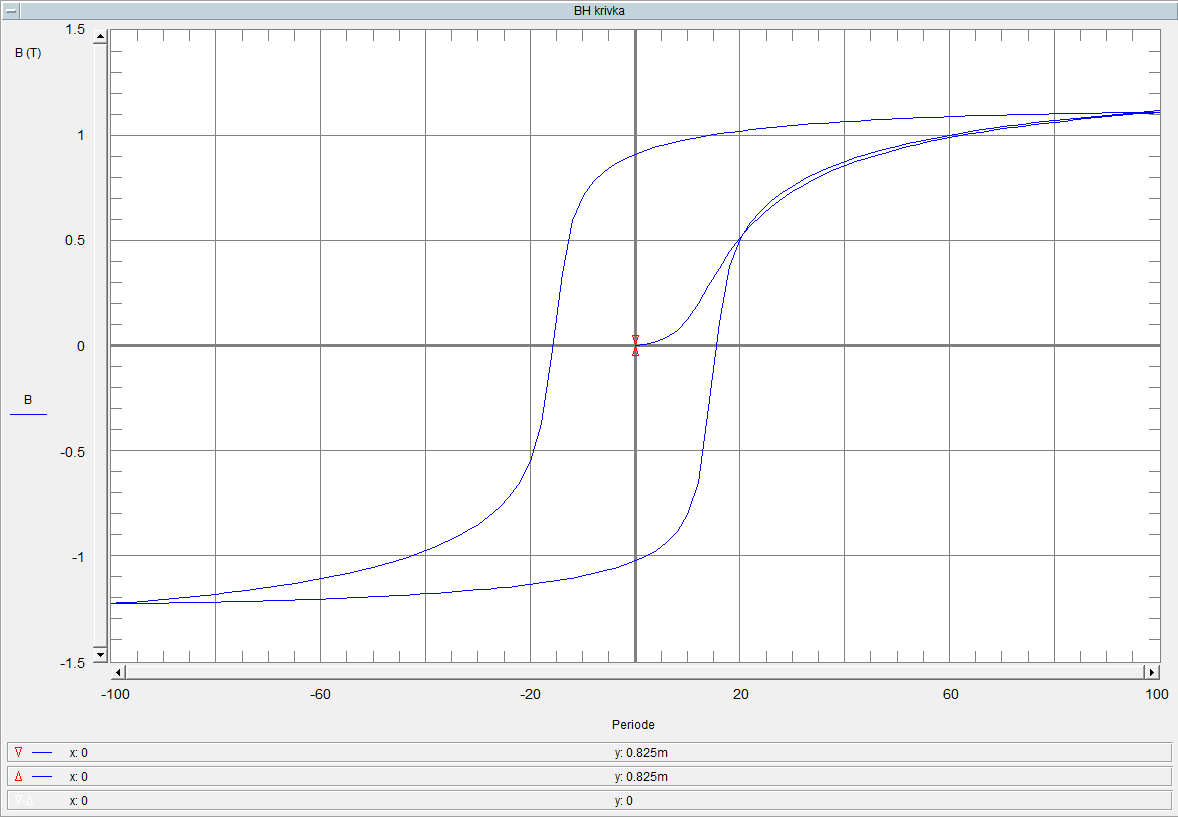
\includegraphics[width=0.9\textwidth]{mag_krivka.png}};
        \draw (0.64,0.87) coordinate(plotCenter);
        \draw[densely dashed, red] (plotCenter) to +(46.2:5);
        \draw[purple, thick] (plotCenter) +(46.2:4) coordinate(bodik) node[plain crossing, rotate=45, scale=0.8]{};
        \draw[{Straight Barb[angle'=60, scale=2]}-{Straight Barb[angle'=60, scale=2]}, red] (bodik) to node[anchor=west]{$\Delta_{\text{B1}}$} +(0,-2.9) coordinate(X);
        \draw[densely dashed, red] (X) to +(0,-4.35);
        \draw[{Straight Barb[angle'=60, scale=2]}-{Straight Barb[angle'=60, scale=2]}, red] (bodik) to node[anchor=south]{$\Delta_{\text{H1}}$} +(-2.8,0) coordinate(X);
        \draw[densely dashed, red] (X) to +(-7.19,0);
    \end{circuitikz}
    \caption{Naměřená hysterezní smyčka měřeného jádra; $\Delta_{B1} = 1\,\text{T}$; $\Delta_{H1} = 38,57\,\text{A}\cdot\text{m}^{-1}$}
\end{figure}

\subsection{Příklady výpočtu}

\begin{enumerate}
    \item Střední délka magnetické siločáry
    \begin{multline*}
        l_\text{s} = \textcolor{teal}{\pi \cdot \frac{d_1 + d_2}{2}} = \pi \cdot \frac{70 \cdot 10^{-3}\,\text{m} + 110 \cdot 10^{-3}\,\text{m}}{2} = 282,7 \cdot 10^{-3}\,\text{m} = \underline{\underline{282,7\,\text{mm}}} \hfill
    \end{multline*}
    \item Průřez předloženého vzorku
    \begin{multline*}
        S_\text{z} = \textcolor{teal}{\frac{d_2 - d_1}{2} \cdot h} = \frac{110 \cdot 10^{-3}\,\text{m} - 70 \cdot 10^{-3}\,\text{m}}{2} \cdot 20 \cdot 10^{-3}\,\text{m} = 400 \cdot 10^{-6}\,\text{m}^2 = \underline{\underline{400\,\text{mm}^2}} \hfill
    \end{multline*}
    \item Maximální velikost magnetického toku
    \begin{multline*}
        \Phi_{\text{max}} = \textcolor{teal}{B_\text{max} \cdot S_\text{z} \cdot N_2} = 1,5\,\text{T} \cdot 400 \cdot 10^{-6}\,\text{m}^2 \cdot 50 = 30 \cdot 10^{-3}\,\text{Wb} = \underline{\underline{30\,\text{mWb}}} \hfill
    \end{multline*}
    \item{Konstanta Wb-metru}
    \begin{multline*}
        k_\Phi = \frac{\Phi_{\text{max}}}{10\,\text{V}} = \frac{30 \cdot 10^{-3}\,\text{Wb}}{10\,\text{V}} = 3 \cdot 10^{-3}\,\text{Wb/V} = \underline{\underline{3\,\text{mWb/V}}} \hfill
    \end{multline*}
    \item Maximální hodnota relativní permeability toroidního vzorku Sonapermu
    \begin{multline*}
        \mu_\text{max} = \textcolor{teal}{\frac{1}{\mu_0} \cdot \frac{\Delta_{B1}}{\Delta_{H1}}} = \frac{1}{4 \pi \cdot 10^{-7}\,\text{H}\cdot\text{m}^{-1}} \cdot \frac{1\,\text{T}}{38,57\,\text{A}\cdot\text{m}^{-1}} = \underline{\underline{20\,631,96}} \hfill
    \end{multline*}
\end{enumerate}

\section{Seznam použitých přístrojů}

\begin{itemize}
    \item Měřící ústředna Agilent 34970A, v.č. MY44004873
    \item Počítač vybaven programem HP VEE
    \item Elektronický fluxmetr
    \item Zdroj magnetizačního proudu
    \item Laboratorní přípravek s měřeným jádrem
\end{itemize}

\section{Závěr}

Úkolem tohoto námi provedeného měření bylo změřit statickou hysterezní smyčku předloženého feromagnetického toroidního jádra pomocí automatizovaného měřícího pracoviště.

Naměřená hysterezní smyčka námi měřeného feromagnetického sonapremového toroidního jádra je uvedena v grafu výše.
Výsledné hodnoty tohoto měření byly uvedeny do výše uvedené přehledné tabulky.

Z námi naměřených hodnot a charakteristik vyplývá, že námi měřený vzorek je zkonstruován z magneticky měkkého materiálu.
Magneticky tvrdé materiály mají totiž mnohonásobně vyšší velikosti hodnot koercivní síly $H_\text{c}$.

Námi měřený vzorek projevoval vlastnosti snadné magnetizace a demagnetizace, což je dalším jevem, že se jedná o magneticky měkký materiál.
Měření magneticky tvrdého materiálu by trvalo násobně déle, jelikož domény v krystalické mřížce magneticky tvrdých materiálů mají tendenci se nevracet do svých původních stavů.

Značný vliv na nepřesnost námi provedeného měření mohlo mít zejména odečítání a odhadování hodnot z naměřené hysterezní smyčky.

\end{document}